\section{سوال ششم - پروژه عملی}


در ادامه پروژه قبلی دو لایه مخفی کاملاً متصل را به سیستم خود متصل کنید. علاوه بر این یک لایه خروجی با ۱۰ نورون نیز برای خروجی شبکه در نظر گرفته و به شبکه متصل شود.



\begin{enumerate}
	\item عملکرد شبکه کاملاً متصل را به صورت مستقل بررسی کنید.
	\item در صورتی که شبکه مشابه در پایتون آموزش داده شده و وزن‌های آن برای تست شبکه در نظر گرفته شود، ۱۰\% امتیاز بیشتر برای بخش پروژه در نظر گرفته می‌شود.
	\item در صورتی که کل شبکه (شامل لایه‌های کانولووشن و کاملاً متصل) در پایتون آموزش داده شده و وزن‌های آن برای تست شبکه در نظر گرفته شود ۲۰\% امتیاز بیشتر برای بخش پروژه در نظر گرفته می‌شود.
\end{enumerate}

	
	در صورت انجام «۲» یا «۳» نیازی به انجام بخش «۱» نمی‌باشد.
	

\begin{qsolve}
	در این پروژه قصد داریم تا پروژه‌های قبلی را با اضافه نمودن یک لایه \lr{Fully Connected} به آن تکمیل کرده و یک شبکه عصبی \lr{CNN} را پیاده‌سازی کنیم. بدین منظور پروژه را به دو فاز تقسیم می‌کنیم:
	\begin{enumerate}
		\item فاز نرم‌افزاری
		\item فاز سخت‌افزاری
	\end{enumerate}
	
	\paragraph{فاز نرم‌افزاری:}
	
	در مرحله اول ابتدا به‌صورت نرم افزاری شبکه مورد نظر را تعریف کرده و آن را با داده‌های مجموعه داده \lr{MNIST} آموزش می‌دهیم تا از وزن‌های آن در فاز سخت افزاری استفاده کنیم.
	
	بدین منظور شبکه ای با معماری زیر را تعریف می‌کنیم:
	
	\begin{center}
		\includegraphics*[width=0.6\linewidth]{pics/img2.pdf}
		\captionof{figure}{معماری شبکه مورد نظر}
		\label{معماری شبکه مورد نظر}
	\end{center}

	کد نوشته شده برای پیاده سازی شبکه به‌صورت زیر است:
\end{qsolve}

	
\begin{latin}
\begin{lstlisting}[language=Python,caption={Model Definition}]
	
def define_model() -> Sequential:
	# Define model.
	model = Sequential()
	model.add(ZeroPadding2D(padding=pad, input_shape=(input_size[0],
			 input_size[1], 1), name="padding_layer"))
	model.add(Conv2D(conv_filter_num, conv_kernel_size, activation="relu",
			 padding="valid", kernel_initializer="he_uniform",
			 input_shape=(30, 30, 1), name="convolution_layer"))
	model.add(MaxPooling2D(pool_size, name="max_pooling_layer"))
	model.add(Flatten(name="flatten_layer"))
	model.add(Dense(10, activation="softmax", name="dense_layer"))
	# Compile model.
	model.Compile(optimizer=Adam(), loss="categorical_crossentropy",
			 metrics=["accuracy"])
	# Return model.
	return model
	
\end{lstlisting}
\end{latin}


\begin{qsolve}
	با کامپایل کردن مدل نوشته شده خروجی شبکه تعریف شده به‌صورت زیر می‌شود:
	
	\begin{center}
		\includegraphics*[width=0.7\linewidth]{pics/img3.png}
		\captionof{figure}{ساختار شبکه تعریف شده}
		\label{ساختار شبکه تعریف شده}
	\end{center}
	
	
	پس از تعریف ساختار شبکه، شبکه را با استفاده از دیتاست \lr{MNIST} در ۵ \lr{Epoch} آموزش می‌دهیم. که نمودار \lr{Loss} و \lr{Accuracy} شبکه برای داده‌های \lr{Train} و \lr{Validation} به‌صورت زیر به‌دست می‌آید:
	
\end{qsolve}

\begin{qsolve}
	\begin{center}
		\includegraphics*[width=0.7\linewidth]{pics/img4.png}
		\captionof{figure}{نمودارهای \lr{Loss} و \lr{Accuracy}}
		\label{نمودارهای Loss و Accuracy}
	\end{center}
	
	دقت شبکه بر روی داده‌های آموزش و تست به ترتیب ۰٫۹۸۱۷ و ۰٫۹۸۰۱ به‌دست آمده است.
	
	همچنین زمان انجام فاز \lr{Inference} نرم‌افزاری برای ۱۰۰ داده از مجموعه داده \lr{MNIST}، ۴۶٫۸۰۷۲ میلی‌ثانیه به‌دست آمده است.
	
	در نهایت تمامی وزن‌ها و پارامتر‌های مورد نیاز شبکه برای فاز سخت‌افزاری را در ۳ فایل با نام‌های:
	
	\begin{latin}
		\begin{itemize}
			\item 
			\texttt{conv\_weights.h}
			
			\item 
			\texttt{dense\_weights.h}
			
			\item 
			\texttt{definitions.h}
		\end{itemize}
	\end{latin}
	
	ذخیره می‌کنیم. فایل \texttt{conv\_weights.h} شامل وزن‌های به‌دست آمده از لایه‌های کانولوشن، فایل \texttt{dense\_weights.h} نیز شامل وزن‌های لایه \lr{Fully Connected} و فایل \texttt{definitions.h} شامل برخی از ضرایب ثابت مورد استفاده در فاز سخت‌افزاری است.
	
	در ادامه تمامی داده‌های تست \lr{MNIST} شامل تصاویر و \lr{Label} های مربوط به آن را در دو فایل \texttt{in.dat} و \texttt{out.dat} ذخیره می‌کنیم. مراحل انجام به طور کامل در فایل \texttt{gen\_data.ipynb} مشخص شده است.

\end{qsolve}



\begin{qsolve}
	\paragraph{فاز سخت‌افزاری:}
	
	در این فاز نیاز است کد لایه \lr{Fully Connected} را نوشته و به به کد کانولوشن قبلی اضاف می‌کنیم و همان ساختار ارائه شده در فاز نرم‌افزاری را در اینجا پیاده‌سازی می‌کنیم.
	
	کد لایه \lr{Fully Connected} به‌صورت زیر ارائه می‌شود:
\end{qsolve}


\begin{latin}
\begin{lstlisting}[language=C,caption={HLS Implementation of Dense Layer}]
	
void dense(hls::stream<float> & flat_to_dense_stream, int filter,
		   hls::stream<float> & dense_to_softmax_stream)
{
	float flat_value;
	float dense_array[DENSE_SIZE] = { 0 };
	
	dense_for_flat:
	for (int i = 0; i < FLAT_SIZE / FILTERS; ++i)
	{
		flat_value = flat_to_dense_stream.read();
		
		for (int d = 0; d < DENSE_SIZE; ++d)
		{
			int index = filter * (FLAT_SIZE / FILTERS) + i;
			dense_array[d] += dense_weights[index][d] * flat_value;
		}
	}
	
	for (int j = 0; j < DENSE_SIZE; ++j)
	{
		dense_to_softmax_stream.write(dense_array[j]);
	}
}

\end{lstlisting}
\end{latin}



\begin{qsolve}
	در این طراحی از ۴ لایه کانولوشن به‌صورت زیر استفاده شده است:
\end{qsolve}



\begin{latin}
\begin{lstlisting}[language=C,caption={HLS Implementation of Convolution Layers}]

void convolutional_layer(
	float pad_img0 [PAD_IMG_ROWS][PAD_IMG_COLS],
	float pad_img1 [PAD_IMG_ROWS][PAD_IMG_COLS],
	float pad_img2 [PAD_IMG_ROWS][PAD_IMG_COLS],
	float pad_img3 [PAD_IMG_ROWS][PAD_IMG_COLS],
	hls::stream<float> conv_to_pool_streams [FILTERS] )
{
	convolution(pad_img0, 0, conv_to_pool_streams[0]);
	convolution(pad_img1, 1, conv_to_pool_streams[1]);
	convolution(pad_img2, 2, conv_to_pool_streams[2]);
	convolution(pad_img3, 3, conv_to_pool_streams[3]);
}
	
\end{lstlisting}
\end{latin}



\begin{qsolve}
	همچنین برای \lr{Flat} کردن \lr{Feature Map} های به‌دست آمده از خروجی لایه‌های کانولوشنی، ماژولی به‌نام \texttt{flattening} به‌صورت زیر تعریف شده است:
\end{qsolve}



\begin{latin}
\begin{lstlisting}[language=C,caption={HLS Implementation of Flatten Layers}]
	
void flattening(hls::stream<float> &  pool_to_flat_stream,
 				hls::stream<float> & flat_to_dense_stream)
{
	flat_for_rows:
	for(int r = 0; r < POOL_IMG_ROWS; ++r)
	{
		flat_for_cols:
		for(int c = 0; c < POOL_IMG_COLS; ++c)
		{
			flat_to_dense_stream.write(pool_to_flat_stream.read());
		}
	}
}
\end{lstlisting}
\end{latin}



\begin{qsolve}
	همچنین ماژول‌های دیگری برای انجام عملیات‌هایی مانند \lr{Zero Padding}، \lr{Pooling}، \lr{Normalization} و ... تعریف شده است که به‌علت طولانی نشدن گزارش آورده نشده است. درنهایت تاپ ماژول طراحی به‌نام \lr{CNN} به‌صورت زیر تعریف شده است:

\end{qsolve}



\begin{latin}
\begin{lstlisting}[language=C,caption={HLS Implementation of \texttt{CNN} Top Module}]

void cnn(float img_in[IMG_ROWS][IMG_COLS], float prediction[DIGITS])
{
	/******** Pre-processing data. ********/
	
	float pad_img0 [PAD_IMG_ROWS][PAD_IMG_COLS] = { 0 };
	normalization_and_padding(img_in, pad_img0);
	
	#if 0
		#ifndef __SYNTHESIS__
			printf("Padded image.\n");
			print_pad_img(pad_img);
		#endif
	#endif
	
	/* Allow parallelism cloning the padded image. */
	float pad_img1 [PAD_IMG_ROWS][PAD_IMG_COLS];
	float pad_img2 [PAD_IMG_ROWS][PAD_IMG_COLS];
	float pad_img3 [PAD_IMG_ROWS][PAD_IMG_COLS];
	
	float value;
	
	clone_for_rows:
	for (int i = 0; i < PAD_IMG_ROWS; ++i)
		clone_for_cols:
		for (int j = 0; j < PAD_IMG_COLS; ++j)
		{
			pad_img1[i][j] = pad_img0[i][j];
			pad_img2[i][j] = pad_img0[i][j];
			pad_img3[i][j] = pad_img0[i][j];
		}
	
	/* Parallel executions start here. */
	dataflow_section(pad_img0, pad_img1, pad_img2, pad_img3, prediction);
}

\end{lstlisting}
\end{latin}




\begin{qsolve}
	درنهایت ماژول \texttt{CNN} را سنتز می‌کنیم. گزارشات سنتز شبکه به‌صورت زیر ارائه می‌شود:
	
	\begin{center}
		\includegraphics*[width=1\linewidth]{pics/Synthesis_Result_1.png}
		\captionof{figure}{منابع مصرفی پس‌از سنتز (الف)}
		\label{منابع مصرفی پس‌از سنتز (الف)}
	\end{center}
	
	
	\begin{center}
		\includegraphics*[width=1\linewidth]{pics/Synthesis_Result_2.png}
		\captionof{figure}{منابع مصرفی پس‌از سنتز (ب)}
		\label{منابع مصرفی پس‌از سنتز (ب)}
	\end{center}
	
	
	\begin{center}
		\includegraphics*[width=1\linewidth]{pics/Synthesis_Result_3.png}
		\captionof{figure}{منابع مصرفی پس‌از سنتز (ج)}
		\label{منابع مصرفی پس‌از سنتز (ج)}
	\end{center}
	
	
	درنهایت فایل \lr{test bench} ای برای طراحی نوشته شده است که ۱۰۰ تصویر ابتدایی را از فایل تصاویر تولید شده در فاز قبل را بخواند و برای پردازش به شبکه بدهد. و خروجی شبکه میزان دقت تشخیص اعداد و زمان مصرف شده به‌ازای تمام فرایند می‌باشد.
\end{qsolve}
\newpage


\begin{qsolve}
	برای مثال، شبکه ما ۱۰۰ تصویر ابتدایی از مجموعه داده‌های تست دیتاست \lr{MNIST} را با دقت ۱۰۰٪ تشخیص می‌دهد:
	
	\begin{center}
		\includegraphics*[width=1\linewidth]{pics/output_predict_100.png}
		\captionof{figure}{\lr{Accuracy} پیش‌بینی به‌ازای ۱۰۰ تصویر}
		\label{Accuracy پیش‌بینی به‌ازای ۱۰۰ تصویر}
	\end{center}
	
	شبکه ما فاز \lr{Inference} را به ازای ۱۰۰ تصویر در ۴٫۴۵ میلی‌ثانیه انجام داده است. درصورتی که در فاز نرم‌افزاری همین تعداد تصویر در مدت زمان ۴۶٫۸۰ میلی‌ثانیه انجام شده است.
	
	
	هرچه تعداد تصاویر را زیاد کنیم دقت شبکه کم می‌شود. برای مثال به ازای ۵۰۰ تصویر دقت تشخیص شبکه ۹۹ درصد به‌دست می‌آید.
	
	\begin{center}
		\includegraphics*[width=1\linewidth]{pics/output_predict_500.png}
		\captionof{figure}{\lr{Accuracy} پیش‌بینی به‌ازای ۵۰۰ تصویر}
		\label{Accuracy پیش‌بینی به‌ازای ۵۰۰ تصویر}
	\end{center}
	
	در این حالت شبکه ۵ تصویر زیر را به اشتباه تشخیص داده است:
\end{qsolve}
\newpage


\begin{figure}[htbp]
	\centering
	% Row 1
	\begin{subfigure}[b]{0.2\linewidth}
		\includegraphics*[width=1\linewidth]{pics/wrong_output_predict0.png}
		\captionof{figure}{تشخیص اشتباه عدد ۰}
		\label{fig:sub1}
	\end{subfigure}
	\hfill
	\begin{subfigure}[b]{0.2\linewidth}
		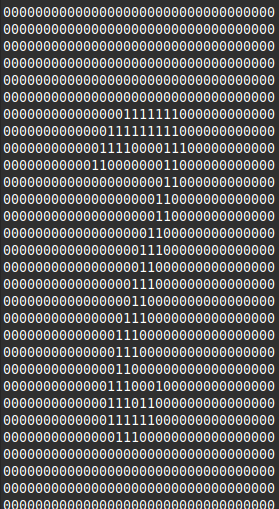
\includegraphics[width=1\linewidth]{pics/wrong_output_predict2.png}
		\captionof{figure}{تشخیص اشتباه عدد ۲}
		\label{fig:sub2}
	\end{subfigure}
	\hfill
	\begin{subfigure}[b]{0.2\linewidth}
		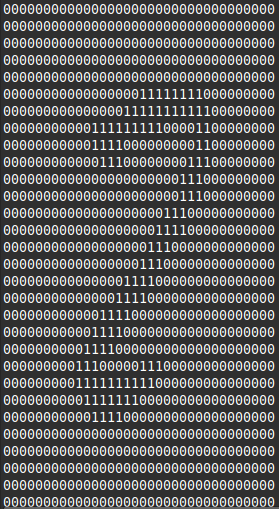
\includegraphics[width=1\linewidth]{pics/wrong_output_predict2_2.png}
		\captionof{figure}{تشخیص اشتباه عدد ۲}
		\label{fig:sub3}
	\end{subfigure}
	
	% Row 2
	\vspace{0.5cm}
	\begin{subfigure}[b]{0.2\linewidth}
		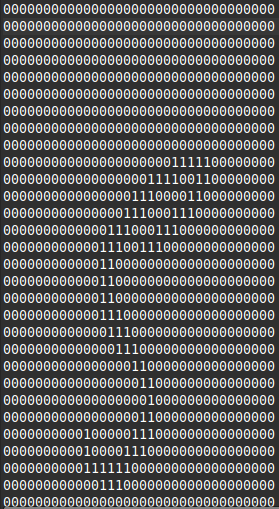
\includegraphics[width=1\linewidth]{pics/wrong_output_predict5.png}
		\captionof{figure}{تشخیص اشتباه عدد ۵}
		\label{fig:sub4}
	\end{subfigure}
	\hfill
	\begin{subfigure}[b]{0.2\linewidth}
		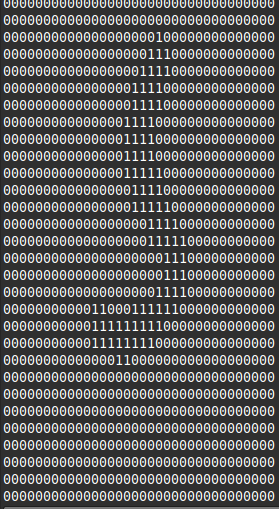
\includegraphics[width=1\linewidth]{pics/wrong_output_predict5_2.png}
		\captionof{figure}{تشخیص اشتباه عدد ۵}
		\label{fig:sub5}
	\end{subfigure}
	
	\captionof{figure}{تشخیص‌های اشتباه شبکه}
	\label{تشخیص‌های اشتباه شبکه}
\end{figure}


\begin{qsolve}
	مقادیری که شبکه برای هر خروجی اشتباه به‌دست آورده است نیز به‌صورت زیر ارائه می‌شود:
\begin{latin}
\noindent\begin{multicols}{3}
\texttt{%
	Prediction for A:\\
	0: 0.000014\\
	1: 0.000002\\
	2: 0.000000\\
	\hl{3: 0.806685}\\
	4: 0.001617\\
	5: 0.037086\\
	6: 0.000001\\
	7: 0.000960\\
	8: 0.003560\\
	9: 0.150075
}

\vfill % Optional spacing

\texttt{%
	Prediction for B:\\
	0: 0.000006\\
	1: 0.000024\\
	2: 0.078408\\
	3: 0.048098\\
	4: 0.000000\\
	5: 0.000003\\
	6: 0.000000\\
	\hl{7: 0.596224}\\
	8: 0.271232\\
	9: 0.006006
}

\vfill % Optional spacing

\texttt{%
	Prediction for C:\\
	0: 0.268470\\
	1: 0.006770\\
	2: 0.000006\\
	3: 0.000007\\
	4: 0.025127\\
	5: 0.002049\\
	6: 0.006413\\
	\hl{7: 0.627097}\\
	8: 0.047987\\
	9: 0.016075
}
\end{multicols}
\end{latin}
	
\end{qsolve}



\begin{qsolve}
\begin{latin}
\noindent\begin{multicols}{2}
	\texttt{%
		Prediction for D:\\
		0: 0.000006\\
		1: 0.005681\\
		2: 0.000050\\
		\hl{3: 0.955743}\\
		4: 0.000271\\
		5: 0.037680\\
		6: 0.000232\\
		7: 0.000000\\
		8: 0.000259\\
		9: 0.000077
	}
	
	
	\texttt{%
		Prediction for E:\\
		0: 0.000000\\
		1: 0.000000\\
		2: 0.137538\\
		3: 0.003166\\
		4: 0.000000\\
		5: 0.000000\\
		6: 0.000000\\
		7: 0.000023\\
		\hl{8: 0.859272}\\
		9: 0.000001
	}
\end{multicols}
\end{latin}
\end{qsolve}


